\section{Diodes}\label{sec:Diodes}
A \nameref{def:Diode} is one of the basic building blocks for almost all analog circuit systems.

\begin{definition}[Diode]\label{def:Diode}
  A \emph{diode} is a 2-port non-linear circuit element.
  Its circuit symbol is shown in \Cref{fig:Diode_Circuit_Symbol}.
\end{definition}

\begin{figure}[h!tbp]
  \centering
  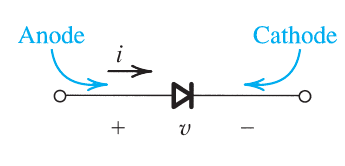
\includegraphics[scale=0.75]{./Diode_Circuit_Symbol.png}
  \caption{Diode Circuit Symbol \parencite[p.~177]{sedraTextbook7}}
  \label{fig:Diode_Circuit_Symbol}
\end{figure}

An \textbf{ideal diode} is one that behaves as a short-circuit when a voltage applied is forward-biased, and acts as an open-circuit with the voltage is reverse-biased.
The current-voltage characteristic is shown in \Cref{fig:Ideal_Diode_IV_Characteristic}.

\begin{figure}[h!tbp]
  \centering
  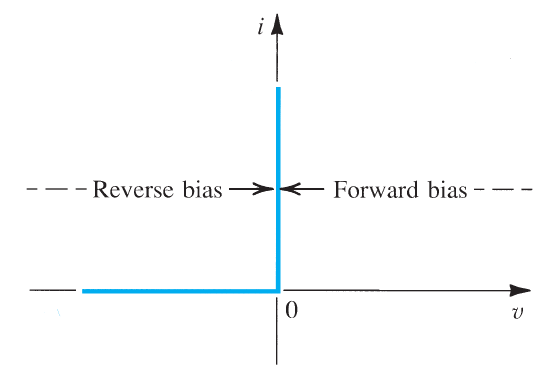
\includegraphics[scale=0.75]{./Ideal_Diode_IV_Characteristic.png}
  \caption{Ideal Diode \DCCurrent{}-\DCVoltage{} Characteristic \parencite[p.~177]{sedraTextbook7}}
  \label{fig:Ideal_Diode_IV_Characteristic}
\end{figure}

\subsection{Terminal Characteristics of Junction Diodes}\label{subsec:Terminal_Characteristics_Junction_Diodes}
A \textbf{junction diode} is a \nameref{def:Diode} built using a \PNJunction{}.
In this case, there are three distinct regions in the characteristic curve:
\begin{enumerate}[noitemsep]
\item \nameref{subsubsec:Diode_Forward-Bias_Region}, where $\Voltage > 0$.
\item \nameref{subsubsec:Diode_Reverse-Bias_Region}, where $\Voltage < 0$.
\item \nameref{subsubsec:Diode_Breakdown_Region}, where $\Voltage < - \ReverseBreakdownVoltage$.
\end{enumerate}


%%% Local Variables:
%%% mode: latex
%%% TeX-master: "../ECE_311-Engineering_Electronics-Reference_Sheet"
%%% End:
